\documentclass[12pt,a4paper,titlepage]{article}
% $Id: example-techreport.tex 1568 2012-11-20 16:01:57Z foley $
% I can comment things out so that the compiler ignores them by using
% these % symbols.  They comment everything after the symbol
% If I want to put % into my text, I need to do this: \%
% I also need to be careful about using other characters like &, which
% will cause problems.
% If there is an error, usually putting the \  in front will fix it.

\usepackage{setspace}
% Create \onehalfspacing command which will set spacing to 1.5

% the \usepackage{}  lines allow me to make use of code other people
% have written.  The ones that are most commonly found just need
% \usepackage{}.  Others may need you to install the package.
% the things in [] square brackets are options to the packages
\usepackage[utf8]{inputenc}  % this allows latex to understand UTF
                             % encoding in the file. This is
                             % important for Icelandic characters.
%\usepackage[icelandic]{babel} % this makes figures and tables have
%their Icelandic names
\usepackage[T1]{fontenc} % this enables icelandic characters in the output

\usepackage{amsmath} % these let you make neat equations.  AMS is the
                     % American Math Society
\usepackage{amsfonts}
\usepackage{amssymb}
\usepackage[amssymb]{SIunits}

% this allows us to format units correctly
% we need the amssymb option to avoid conflict on \square
%\usepackage[amssymb]{siunitx}

% this creates the Pseudocode environment for algorithms
\usepackage{pseudocode}

% this allows me to include code snippets and make them pretty
\usepackage{listings}

% this allows me to adjust the margins
\usepackage[left=2.00cm, right=2.00cm, top=2.00cm, bottom=2.00cm]{geometry}


%\usepackage[today,fancyhdr]{svninfo} % grab the SVN revision information
% This package allows you to include svn information into your document
% You will need to set the svn:keywords property to have Id and HeadURL for it to work.
%% The ``today'' option sets the current day to the latest SVN date
%
%\setlength{\headheight}{15pt} % to make fancyhdr not give a warning
%% These lines are filled in by SVN if you set the keywords
%\svnInfo $Id: example-techreport.tex 1568 2012-11-20 16:01:57Z foley $
%\svnKeyword $HeadURL: https://projects.cs.ru.is/svn/mechatronics1-2012/Templates/LaTeX-TechReport/example-techreport.tex $
%\pagestyle{fancyplain}
%% This avoids putting the information on the first page

\usepackage{graphicx}
% this package allows \includgraphics to work for putting pictures in
% the document.  The older version is graphics, you should use
% graphicx instead.

\usepackage{url}
% this package allows URLs, which show up in the bibliography and
% possibly elsewhere.  you use it like this: \url{www.google.com}

\usepackage{hyperref}
% Make magic hyperlink

\author{Páll Helgason pallsh12@ru.is\\Sindri Ólafsson sindrio12@ru.is\\Sveinn Elmar Magnússon sveinnm12@ru.is\\Þór Tómasarson thortom12@ru.is}  % My name, for the titlepage
\title{
\includegraphics{graphics/ru-logo}\\\vspace{10mm}
T-411-MECH Mechatronics 1\\Data logger for geological research\\Team Proposal}  % The title, for the titlepage


\begin{document} % this tells the compiler that it is time to make
                 % text to print instead of just getting ready.
\maketitle  % make a title page from the Title, Date, and Author
\onehalfspacing % 1.5 spacing

This report is a proposal of a mechatronic project to do as a
final project in the course T-411-MECH Mechatronics for the fall of 2014.
 

\section{Description}
Andrew Wickert is a PHD in earth surface processes in University of Colorado and has an 
idea of using the Arduino platform as a base for low-cost data logger used mainly
for geological research. The Arduino platform offers a wide range of application and connection to 
sensors. The Arduino community provides large collection of libraries and various vendors have 
variety of shields for all kind of application. 
Available WSN platform \cite{WSN} to day for harsh and remotely areas are heavy and expensive.
Arduino platform offers opportunity to make low-cost WSN platform.
This project aims first at making a solid means of communication between data-loggers and mother hub
and secondly of good power-management for the logger. 


\section{Application}

The main application of the data logger will be telemetry for returning data. Good telemetry communication for a data logger eases the process of maintenance checks and enables more involved researches.\\
Telemetry via GSM network is available throughout most part of Iceland, see figure~\ref{fig:GSM-Coverage}. With GSM shield on the data logger one might be able to monitor data logging in most places in Iceland.\\
Radio coverage can be quite good over long distance. The XBee modules with Arduino support come with radio ranges for up to 60km \cite{Xbee}. If the data logger is equipped with the Xbee module the researcher might set up a ground station with in a 60km radius.\\
Satellite phone (Iridium) might be connected to the data logger to enable good coverage in remote areas. Iridium phone has coverage anywhere in the world were there is a clear view of the sky, by connecting to any of the 66 iridium satellites in orbit around the earth\cite{iridium}. We will try to make standard platform for GSM, Xbee and Iridium. So it will be easy to switch between modules like in figuree~\ref*{fig:Inside} 

\begin{figure}
\centering
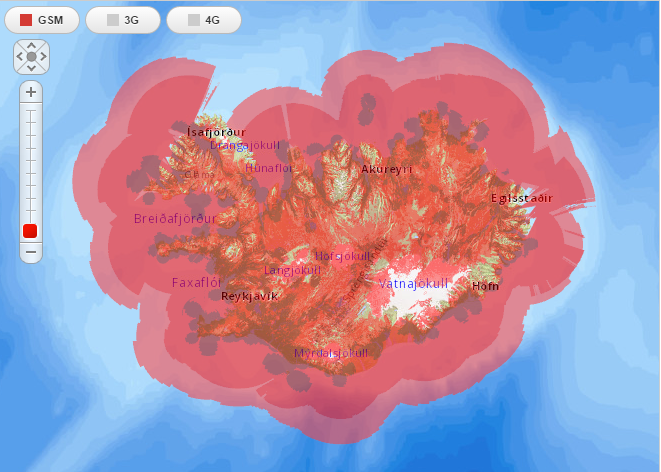
\includegraphics[height=50mm]{graphics/GSM_Coverage.PNG}
\caption{GSM coverage in Iceland\label{fig:GSM-Coverage} \cite{vodafone}}
\end{figure}

\begin{figure}
\centering
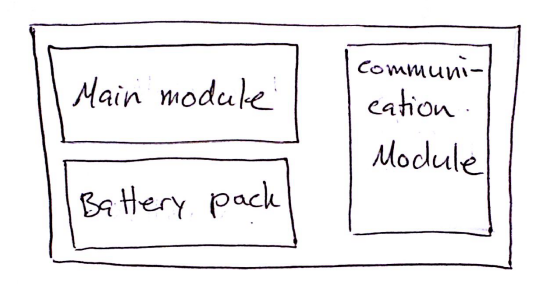
\includegraphics[height=50mm]{graphics/Inside_box.PNG}
\caption{Raw figure of Data Logger inside\label{fig:Inside} \cite{InsideBox}}
\end{figure}

\section{Usage} 

\begin{figure}
\centering
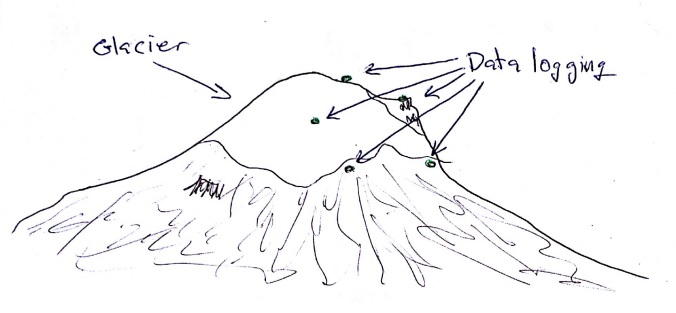
\includegraphics[width=0.7\linewidth]{graphics/Logging}
\caption{Glacier data logging}
\label{fig:glacier}\cite{Helgason_glacier}
\end{figure}

 This equipment useful in geological measurements, mainly for weather and water-resources, see figure~\ref*{fig:glacier}. Especially in remote locations. 
 Geologist Andy Wickert has special interests in this equipment to collect geological data with higher density and wider distribution. 
 


\subsection{Bill of material} % (fold)
\begin{center}
    \begin{tabular}{ | p{1.5cm} | p{1.4cm} | p{1.5cm} | l | p{5cm} | p{5cm} |}
    \hline
    Item & Already have & Quantity & Cost & URL & Summary \\ \hline
    
    Arduino Mega & - & 1x & 45.95\$ & \url{https://www.sparkfun.com/products/11061} & Open-source electronics platform \\ \hline
    
    GSM Module with shield & - & 1x & 99.95\$ & \url{https://www.sparkfun.com/products/9607} & Connects Arduino to the internet using the GPRS wireless network \\ \hline
    
	Special AM board from Andy & - & 4x & $\sim$80\$ & \url{https://github.com/NorthernWidget/ALog-LogMega/blob/FoleyMechatronics/BoM/LogMega083_DigiKey.csv} &  \\ \hline
    \end{tabular}
\end{center}
 

% subsection subsection_name (end)
\bibliographystyle{IEEEtran}
\bibliography{references}

\end{document} % this tells the compiler that we are done=======
